% Derivato dal mio template vecchio e da https://www.overleaf.com/latex/templates/template-tesi-universita-di-pisa/xwjmznxbtszd
%   Il progetto nasce dal template per il frontespizio realizzato da Marco Antonio Corallo, che ringrazio. Seguono alcuni commenti per evidenziare la presenza di alcuni pacchetti che mi sono stati utili per la stesura della tesi. Chiaramente, dipende tutto dal tipo di lavoro che uno vuole eseguire, che determina anche le diverse esigenze. Durante la stesura ho passato molto tempo su siti e forum a cercare di risolvere alcuni probelmi di formattazione, ma in generale Latex è stato piuttosto versatile. 

% Tipo di documento. L'uso di twoside implica che i capitoli inizino sempre con la prima pagina a sinistra, eventualmente lasciando una pagina vuota nel capitolo precedente. Se questa cosa è fastidiosa, è possibile rimuoverlo. 
\documentclass[a4paper, twoside,openright]{report}

% Dimensione dei margini
\usepackage[a4paper,top=3cm,bottom=3cm,left=3cm,right=3cm]{geometry} 
% Dimensione del font
\usepackage[fontsize=13pt]{scrextend}
% Lingua del testo
\usepackage[english]{babel}
% Lingua per la bibliografia
\usepackage[fixlanguage]{babelbib}
% Codifica del testo
\usepackage[utf8]{inputenc} 
% Encoding del testo
\usepackage[T1]{fontenc}
% Permette di generare testo fittizio.
\usepackage{lipsum}
% Per ruotare le immagini
\usepackage{rotating}
% Per modificare l'header delle pagine 
\usepackage{fancyhdr}           

\usepackage{float}
\usepackage{caption}
\usepackage{subcaption}

% Librerie matematiche
\usepackage{amssymb}
\usepackage{amsmath}
\usepackage{amsthm}         

% Uso delle immagini
\usepackage{graphicx}
% Uso dei colori
\usepackage[dvipsnames]{xcolor}         
% Uso dei listing per il codice
\usepackage{listings}          
% Per inserire gli hyperlinks tra i vari elementi del testo 
\usepackage{hyperref}     
% Diversi tipi di sottolineature
\usepackage[normalem]{ulem}

% -----------------------------------------------------------------

% Modifica lo stile dell'header
\pagestyle{fancy}
\fancyhf{}
\lhead{\rightmark}
\rhead{\textbf{\thepage}}
\fancyfoot{}
\setlength{\headheight}{12.5pt}

% Rimuove il numero di pagina all'inizio dei capitoli
\fancypagestyle{plain}{
  \fancyfoot{}
  \fancyhead{}
  \renewcommand{\headrulewidth}{0pt}
}

% Stile del codice
\lstdefinestyle{codeStyle}{
    % Colore dei commenti
    commentstyle=\color{teal},
    % Colore delle keyword
    keywordstyle=\color{Magenta},
    % Stile dei numeri di riga
    numberstyle=\tiny\color{gray},
    % Colore delle stringhe
    stringstyle=\color{violet},
    % Dimensione e stile del testo
    basicstyle=\ttfamily\footnotesize,
    % newline solo ai whitespaces
    breakatwhitespace=false,     
    % newline si/no
    breaklines=true,                 
    % Posizione della caption, top/bottom 
    captionpos=b,                    
    % Mantiene gli spazi nel codice, utile per l'indentazione
    keepspaces=true,                 
    % Dove visualizzare i numeri di linea
    numbers=left,                    
    % Distanza tra i numeri di linea
    numbersep=5pt,                  
    % Mostra gli spazi bianchi o meno
    showspaces=false,                
    % Mostra gli spazi bianchi nelle stringhe
    showstringspaces=false,
    % Mostra i tab
    showtabs=false,
    % Dimensione dei tab
    tabsize=2
} \lstset{style=codeStyle}

% Stile di codice per dimensioni maggiori, in cui ho avuto bisogno di un testo più picolo (ad esempio se si vuole inserire del codice che ha linee molto lunghe). Per usare questo stile piuttosto che il precedente, usare 

% \lstset{style=longBlock}
%  % inserire il codice...
% \lstset{style=codeStyle}

% Il secondo comando consente di tornare allo stile precedente 
\lstdefinestyle{longBlock}{
    commentstyle=\color{teal},
    keywordstyle=\color{Magenta},
    numberstyle=\tiny\color{gray},
    stringstyle=\color{violet},
    basicstyle=\ttfamily\scriptsize,
    breakatwhitespace=false,         
    breaklines=true,                 
    captionpos=b,                    
    keepspaces=true,                 
    numbers=left,                    
    numbersep=5pt,                  
    showspaces=false,                
    showstringspaces=false,
    showtabs=false,                  
    tabsize=2
} \lstset{style=codeStyle}

% Togliendo il commento al comando che segue, si inseriscono nella bibliografia anche le fonti presenti in Bibliography.bib ma non citati direttamente con il comando \cite
% \nocite{*}

% Margini prima e dopo blocchi di codice, per avere più distanza
\lstset{aboveskip=20pt,belowskip=20pt}

% Aggiunti definizioni, teoremi, linea e listing
\newtheorem{definition}{Definizione}[section]
\newtheorem{theorem}{Teorema}[section]
\providecommand*\definitionautorefname{Definizione}
\providecommand*\theoremautorefname{Teorema}
\providecommand*{\listingautorefname}{Listing}
\providecommand*\lstnumberautorefname{Linea}

\raggedbottom

%\newcommand{\cgs}[1]{{\textcolor{brown}[\textcolor{red}{\bf{GS: }}{ \textcolor{brown}{#1]}}}}             
%\newcommand{\cmc}[1]{{\textcolor{blue}[\textcolor{magenta}{\bf{MC: }}{ \textcolor{blue}{#1]}}}}


% -----------------------------------------------------------------
\begin{document}

\begin{titlepage}
\begin{figure}[!htb]
    \centering
    
\includegraphics[keepaspectratio=true,scale=0.5]{figures/logounipg2021}
\end{figure}

\begin{center}
    \LARGE{UNIVERSIT\`A DEGLI STUDI DI PERUGIA}
    \vspace{5mm}
    \\ \Large{Dipartimento di Ingegneria}
    \vspace{5mm}
    \\ \LARGE{Laurea Magistrale in \\ Ingegneria Informatica e Robotica}
\end{center}

\vspace{15mm}
\begin{center}
    {\LARGE{\bf Un fantastico titolo\\ \vspace{5mm} per la mia tesi di laurea! }}
    
    % Se il titolo è abbastanza corto da stare su una riga, si può usare
    
    % {\LARGE{\bf Un fantastico titolo per la mia tesi!}}
\end{center}
\vspace{30mm}

\begin{minipage}[t]{0.47\textwidth}
	{\large{Relatore:}{\normalsize\vspace{3mm}
	\bf\\ \large{Prof. Gabriele Costante} }} %\normalsize\vspace{3mm}\bf \\ \large{Prof: Nome Cognome}
\end{minipage}
\hfill
\begin{minipage}[t]{0.47\textwidth}\raggedleft
	{\large{Candidato:}{\normalsize\vspace{3mm} \bf\\ \large{Paolo Speziali}}}
\end{minipage}

\vspace{30mm}
\hrulefill
\\\centering{\large{Anno Accademico 2023/2024}}

\end{titlepage}

\include{chapters/Abstract}

\tableofcontents

% Rimuovere se non si vuole la tabella delle figure
\listoffigures

\chapter{Introduction}

\section{Data Scarcity and Noisy Datasets in Machine Learning}

\textbf{Machine Learning} (ML) is reshaping our world in ways both
subtle and profound. From the personalized recommendations we receive
on streaming platforms to the autonomous vehicles navigating in real streets,
ML algorithms are becoming an integral part of our daily lives.
Yet, as these systems tackle increasingly complex challenges,
they reveal their limitations.
One of the most pressing issues is the critical need for large, 
high-quality datasets, a requirement that is often difficult to
meet in real-world scenarios.

The \textbf{scarcity} of comprehensive datasets poses a significant
obstacle in many fields, including healthcare and robotics.
In \textbf{healthcare}, privacy concerns and limited access to patient
records hinder the collection of diverse and extensive data.
Similarly, in \textbf{robotics}, certain experimental data may be difficult
or costly to obtain, particularly in scenarios involving complex
physical interactions or rare events. This data scarcity can lead
to underfitted or non-generalizable models, compromising their
accuracy and utility in practical applications.

Moreover, even when substantial datasets are available, they
often suffer from \textbf{noise and inconsistencies}. Real-world data
collection processes are rarely perfect, resulting in datasets
that may contain errors, outliers, or biased samples.
These imperfections can significantly impact the performance of ML models,
leading to unreliable predictions or decisions. The challenge of dealing
with noisy datasets is particularly acute in offline
\textbf{Deep Reinforcement Learning} (DRL) scenarios, where agents must learn
optimal policies from pre-collected experiences without the ability
to interact further with the environment.

To address these challenges, researchers have long employed
\textbf{data augmentation techniques}. Traditional data augmentation
methods involve
applying various transformations to existing data points to artificially
expand the dataset. In image processing, for instance, this might involve
rotations, flips, or color adjustments. While these techniques have proven
effective in many applications, they have limitations.
Notably, not all transformations produce valid or realistic data points,
especially in domains with complex underlying structures or causal relationships.

This is where the integration of \textbf{Causal Inference} into
ML frameworks offers a
promising solution. Causal inference focuses on understanding the
cause-and-effect relationships between variables, rather
than merely identifying correlations. By leveraging causal inference,
we can develop more sophisticated data augmentation techniques that
respect the underlying causal structure of the data-generating process.

In this thesis, we propose novel approaches to address the
challenges of data scarcity and noisy datasets by leveraging
causal inference techniques. We introduce two frameworks for
counterfactual data generation:
the \textbf{Wasserstein Reward-enhanced Counterfactual Data Generation}
(WRe-CTDG) and the \textbf{End-to-End Counterfactual Data Generation} (e2e-CTDG).
These methods aim to augment pre-collected datasets by generating additional
high-fidelity experiences that align with the environment's underlying
transition dynamics.

Our work focuses specifically on offline DRL scenarios, where agents
are trained using pre-collected datasets of experiences.
We explore applications in both robotics environments
(such as Acrobot, Half Cheetah, and Pusher) and healthcare scenarios
(such as diabetes treatment simulation).
These domains present unique challenges due to their complex
dynamics and the potential consequences of incorrect decisions.

By incorporating \textbf{Structural Causal Models} (SCMs) and
\textbf{Generative Adversarial Networks} (GANs) into our frameworks,
we develop techniques to infer causal relationships and generate counterfactual
samples. This approach allows us to create synthetic data points
that are not mere transformations of existing data, but rather plausible
alternative scenarios that could have occurred under different circumstances.
This is particularly valuable in offline DRL, where the ability to explore
``what-if'' scenarios can significantly enhance the robustness
and generalization capabilities of learned policies.

\section{Structure of the Thesis}

The following chapters are organized as follows:
\begin{itemize}
    \item In \textbf{Chapter 2}, we provide an overview of the State of the Art
    in Offline Reinforcement Learning, Data Augmentation and Generation Techniques,
    and Counterfactual Reasoning in Data Generation.
    \item In \textbf{Chapter 3}, we introduce the theoretical foundations
    of the tecnologies used in our proposed frameworks,
    including Structural Causal Models,
    Generative Adversarial Networks,
    and Deep Reinforcement Learning algorithms.
    \item In \textbf{Chapter 4}, we present the WRe-CTDG
    and the e2e-CTDG frameworks,
    detailing their architectures and training procedures.
    We also present the environments and datasets used for evaluation.
    \item In \textbf{Chapter 5}, we present a comprehensive description
    of the machines and neural networks employed in our experiments,
    followed by a detailed overview of the experimental results.
    \item In \textbf{Chapter 6}, we discuss the implications of our findings,
    the limitations of our approaches,
    and potential directions for future research.
\end{itemize}

\chapter{State of the Art}

\chapter{Prior Knowledge}

\section{Deep Learning}

In the field of machine learning, the first models you
are often introduced to are those for regression
and classification that utilize linear
combinations of fixed basis functions.
According to \cite{Bishop:2008aa},
these models possess useful analytical and computational properties,
but their practical applicability is constrained 
since their capacity is limited to linear functions
and they cannot understand the interaction between any two input variables.
This leads to problems such as the curse of dimensionality,
where the number of possible interactions between variables grows exponentially
with the number of input variables.
To address large-scale problems, it is essential to adapt the basis functions
to the data, as demonstrated by support vector machines (SVMs).
Alternatively, one can fix the number of basis functions in advance while
allowing them to be adaptive, utilizing parametric forms for the basis
functions with parameter values adjusted during training.

The most successful example of this approach in pattern recognition is the
\textbf{feed-forward neural network},
also known as the multilayer perceptron (MLP).
\begin{figure}[h]
    \centering
    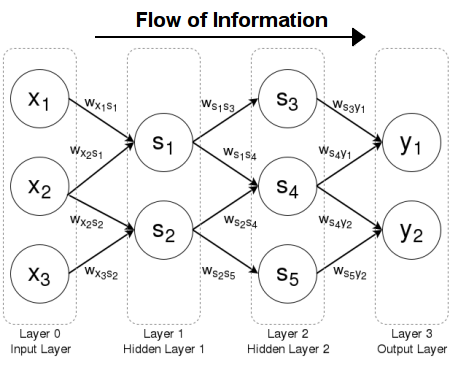
\includegraphics[width=.9\textwidth]{figures/ch3/1.mlp.png}
    \caption{A feed-forward neural network with two hidden layers}
    \vspace{-10px}
    \caption*{\scriptsize{Source: \href{https://brilliant.org/wiki/feedforward-neural-networks/}{Brilliant}}}
    \label{fig:mlp}
\end{figure}

As explained in 
\cite{goodfellow2016deep},
the goal of a feedforward network is to approximate a specific function
\( f^* \). For example, in a classification task,
\( y = f^*(x) \) maps an input \( x \) to a category \( y \).
A feedforward network defines a mapping \( y = f(x; \theta) \) and
learns the parameters \( \theta \) that yield the best approximation
of this function.

These models are called \textbf{feedforward} because information
flows unidirectionally from the input \( x \), through intermediate computations
defining \( f \), and ultimately to the output \( y \), without feedback loops.

The training data directly specifies the output layer's behavior but
not the intermediate layers, which are called \textbf{hidden layers}
because their desired outputs are not provided by the training data.
The learning algorithm must determine how to best utilize these
hidden layers to approximate \( f^* \).
Every layer of the network computes a non-linear transformation of the
previous layer's activations, this way a complex function can be
approximated by composing simpler functions, one for each layer.
Layers are composed of a set of units, where each unit is a node that
computes a non-linear function of the weighted sum of its inputs
and is only connected to units in the previous and the following layer.

A feedforward network is called a \textbf{deep neural network} if it has
more than one hidden layer, the branch of machine learning that studies
deep neural networks is called \textbf{deep learning}.

They are called networks due to their structure, which involves composing
multiple functions together. Typically, this composition is represented
by a directed acyclic graph. For instance, functions
\( f^{(1)} \), \( f^{(2)} \), and \( f^{(3)} \) might be connected in
a chain to form \( f(x) = f^{(3)}(f^{(2)}(f^{(1)}(x))) \).

Functions \( f^{(1)} \) and \( f^{(2)} \) must
be non linear, otherwise the composition would collapse into a single
linear function. These non-linear functions are
called \textbf{activation functions}.
The last function \( f^{(3)} \) is typically a linear function that maps
the output of the final hidden layer to the output layer.
This is the same as applying a linear model to a transformed
input \( \phi(x) \), where \( \phi \) is a nonlinear transformation.
The question then becomes how to choose the mapping \( \phi \).

The strategy of deep learning is to learn \( \phi \):
in this approach, we use a model
\[ y = f(x; \theta, w) = \phi(x; \theta)^\top w \]
Here, we have parameters \( \theta \) that are used to learn \( \phi \)
from a broad class of functions, and parameters \( w \) that map \( \phi(x) \)
to the desired output.
This approach allows for greater flexibility:
specifically, by using a broad family of functions
\( \phi(x; \theta) \), the human designer only needs to select the appropriate
general function family rather than finding precisely an exact function.

The \textbf{universal approximation theorem} \cite{HORNIK1989359}
tells us that regardless of what function
we are trying to learn, we know that a feedforward network with enough units
will be able to \emph{represent} this
function, however we are not guaranteed that the training algorithm will be able
to \emph{learn} it.

\section{Reinformcement Learning}

``\textbf{Reinforcement learning} is learning [...] how
to map situations to actions so
as to maximize a numerical reward signal.
The learner is not told which actions to
take, but instead must discover which actions
yield the most reward by trying them. In
the most interesting and challenging cases, actions may
affect not only the immediate
reward but also the next situation and,
through that, all subsequent rewards.
These two
characteristics, \textbf{trial-and-error search} and \textbf{delayed reward},
are the two most important
distinguishing features of reinforcement learning.'' \cite{sutton1998}

Let's explore the basic concepts of reinforcement learning with
a simple example as described in \cite{zhao2024RLBook}.
Consider a grid world scenario as shown in Figure \ref{fig:rl}
where a robot, referred to as
the \textbf{agent}, moves between cells, occupying one cell at a time.
The white cells are accessible, while the orange cells are forbidden.
The goal is for the agent to reach a target cell.

\begin{figure}[h]
    \centering
    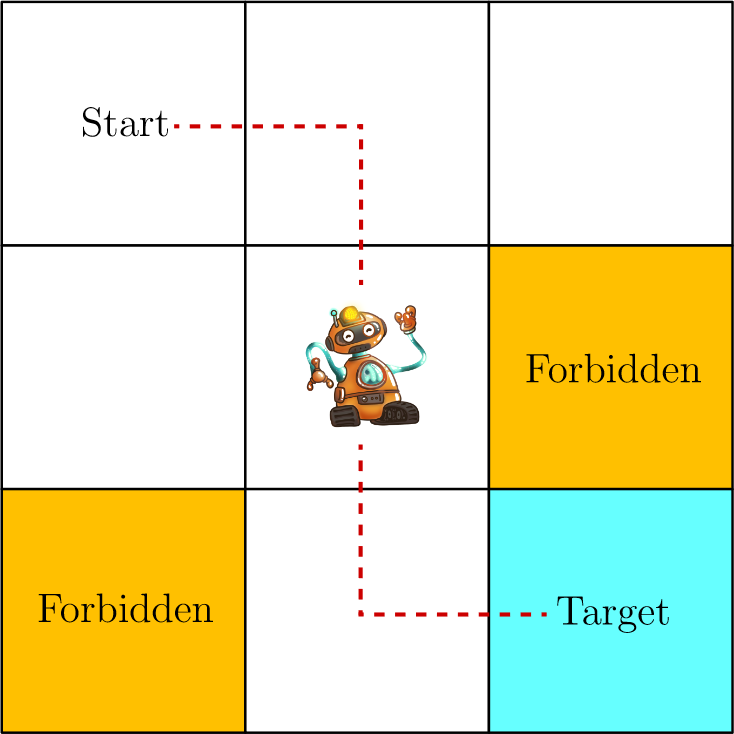
\includegraphics[width=.42\textwidth]{figures/ch3/2.rl.png}
    \caption{A simple reinforcement learning task}
    \vspace{-10px}
    \caption*{\scriptsize{Source: \cite{zhao2024RLBook}}}
    \label{fig:rl}
\end{figure}

To achieve this, the agent needs a \textbf{policy} that guides it to the target
efficiently, avoiding forbidden cells and unnecessary detours.
If the grid layout is known, planning is simple.
However, without prior knowledge, the agent must explore and learn
through trial and error.

The agent's status in the grid is defined by its \textbf{state}
\( s_i \in \mathcal{S} \), which represents its location relative
to the \textbf{environment}.
In the examples with nine cells, the state space is
\( \mathcal{S} = \{s_1, s_2, \ldots, s_9\} \)..

From each state, the agent can perform five \textbf{actions}: move up,
right, down, left or stay put, denoted as \( a_1, a_2, \ldots, a_5 \),
this set of actions is the action space
\( \mathcal{A} = \{a_1, \ldots, a_5\} \).
The available actions can vary by state, for instance,
at \( s_1 \), actions \( a_1 \) (up) and \( a_4 \) (left) would collide
with the grid boundary, so the action space is
\( \mathcal{A}(s_1) = \{a_2, a_3, a_5\} \).

When taking an action, the agent may move from one state to another,
a process known as \textbf{state transition}. For example,
if the agent is at state \( s_1 \) and selects action
\( a_2 \) (moving rightward), it transitions to state
\( s_2 \). This process can be represented as:
\[ s_1 \overset{a_2}{\longrightarrow} s_2 \]
The state transition process is defined for each
state and its associated actions. Mathematically, state transitions
are described by conditional probabilities.
For example, for \( s_1 \) and \( a_2 \),
the conditional probability distribution is:
\[
\begin{aligned}
p(s_1 \mid s_1, a_2) &= 0, \\
p(s_2 \mid s_1, a_2) &= 1, \\
p(s_3 \mid s_1, a_2) &= 0, \\
p(s_4 \mid s_1, a_2) &= 0, \\
p(s_5 \mid s_1, a_2) &= 0,
\end{aligned}
\]
indicating that taking \( a_2 \) at \( s_1 \) guarantees
the agent moves to \( s_2 \), with a probability of one,
and zero probability for other states.

This is a deterministic state transition,
but state transitions can also be stochastic,
requiring conditional probability distributions.
For instance, if random wind gusts affect the grid,
taking action \( a_2 \) at \( s_1 \) might blow the agent to \( s_5 \)
instead of \( s_2 \), resulting in \( p(s_5 \mid s_1, a_2) > 0 \).

A \textbf{policy} is a function that maps states to actions,
indicating the agent's behavior in the environment.
In other words, a policy tells the agent what action to take
at each state.

Mathematically, policies can be described by conditional probabilities.
For example, the policy for \( s_1 \) is:
\[
\begin{aligned}
\pi(a_1 \mid s_1) &= 0, \\
\pi(a_2 \mid s_1) &= 1, \\
\pi(a_3 \mid s_1) &= 0, \\
\pi(a_4 \mid s_1) &= 0, \\
\pi(a_5 \mid s_1) &= 0,
\end{aligned}
\]
indicating that the probability of taking action \( a_2 \) at state \( s_1 \)
is one, and the probabilities of taking other actions are zero.

The above policy is deterministic, but policies may generally be stochastic.
For instance, let's assume that at state \( s_1 \)
the agent may take actions to move either rightward or downward,
each with a probability of 0.5. In this case, the policy for \( s_1 \) is:
\[
\begin{aligned}
\pi(a_1 \mid s_1) &= 0, \\
\pi(a_2 \mid s_1) &= 0.5, \\
\pi(a_3 \mid s_1) &= 0.5, \\
\pi(a_4 \mid s_1) &= 0, \\
\pi(a_5 \mid s_1) &= 0.
\end{aligned}
\]

After executing an action at a state, the agent receives a
reward \( r \) as feedback from the environment.
The \textbf{reward} is a function of the state and action
which predicts immediate reward and is denoted as:
\[ R(s_t=s, a_t=a) = \mathbb{E} [r_t | s_t = s, a_t = a] \]
and it can be positive, negative, or zero.
Different rewards influence the policy the agent learns.
Generally, a positive reward encourages the agent to take the
corresponding action, while a negative reward discourages it.

However we can't find good policies
by simply selecting actions with the greatest immediate rewards
since they do not consider
long-term outcomes. To determine a good policy, we must consider the total
reward obtained in the long run and
an action with the highest immediate reward may not lead to
the greatest total reward.

A \textbf{trajectory} is a state-action-reward chain.
For example, the agent in our example may follow this trajectory:
\[ s_1 \xrightarrow{a_2, r=0} s_2 \xrightarrow{a_3, r=0} s_5 \xrightarrow{a_3, r=0} s_8 \xrightarrow{a_2, r=1} s_9. \]
The \textbf{return} of this trajectory is the sum of all rewards collected along it,
in the example above:
\[\text{return} = 0+0+0+1=1\]
Returns, also called total rewards or cumulative rewards,
are used to evaluate policies.
Returns can also be defined for infinitely long trajectories, which may diverge.
Therefore, we introduce the concept of \textbf{discounted return} for infinitely
long trajectories. The discounted return is the sum of the rewards from $t$ to $T$ (final step):
\[
G_t \doteq R_{t+1} + \gamma R_{t+2} + \gamma^2 R_{t+3} + \ldots = \sum_{k=0}^{\infty} \gamma^k R_{t+k+1}
\]
where \( \gamma \in [0, 1] \) is the \textbf{discount factor}.
If \( \gamma \) is close to 0, the agent emphasizes near-future rewards,
resulting in a short-sighted policy. If \( \gamma \) is close to 1,
the agent emphasizes far-future rewards.

When $T$ is finite, we call the task episodic and each sequence
up to the \textbf{terminal state} is an \textbf{episode}. Otherwise, we refer
to \textbf{continuing tasks}.

The \textbf{Markov Decision Processes} (MDPs),
a general framework for describing stochastic dynamical systems,
allows us to formally presents these concepts.
The \textbf{Markov property} refers to the \textbf{memoryless} property of a stochastic process. Mathematically, it means that
\[
\begin{aligned}
p(s_{t+1} \mid s_t, a_t, s_{t-1}, a_{t-1}, \ldots, s_0, a_0) &= p(s_{t+1} \mid s_t, a_t), \\
p(r_{t+1} \mid s_t, a_t, s_{t-1}, a_{t-1}, \ldots, s_0, a_0) &= p(r_{t+1} \mid s_t, a_t),
\end{aligned}
\]
where \( t \) represents the current time step and \( t + 1 \) represents the next time step.
This indicates that the next state or reward depends only on the current
state and action and is independent of the previous ones.

\vspace{3cm}

An MDP is defined by a tuple \( \langle \mathcal{S}, \mathcal{A}, P, R, \gamma \rangle \),
let's break down the components:
\begin{itemize}
    \item \( \mathcal{S} \): finite set of Markov states $s$
    \item \( \mathcal{A} \): finite set of actions $a$
    \item \( P \): state transition model for each action,
    a probability matrix that specifies $$p(s_t+1 = s'|s_t=s, a_t=a)$$
    \item \( R \): reward function
    $$ R(s_t=s, a_t=a) = \mathbb{E} [r_t | s_t = s, a_t = a] $$
    \item \( \gamma \): discount factor $0 \leq \gamma \leq 1$
\end{itemize}

When the policy in a MDP is fixed, it reduces to a \textbf{Markov Process} (MP),
this transformation simplifies the MDP by eliminating the decision-making aspect. 
A Markov process is referred to as a \textbf{Markov Chain} if it operates in discrete
time and the number of states is either finite or countable.

\begin{figure}[h]
    \centering
    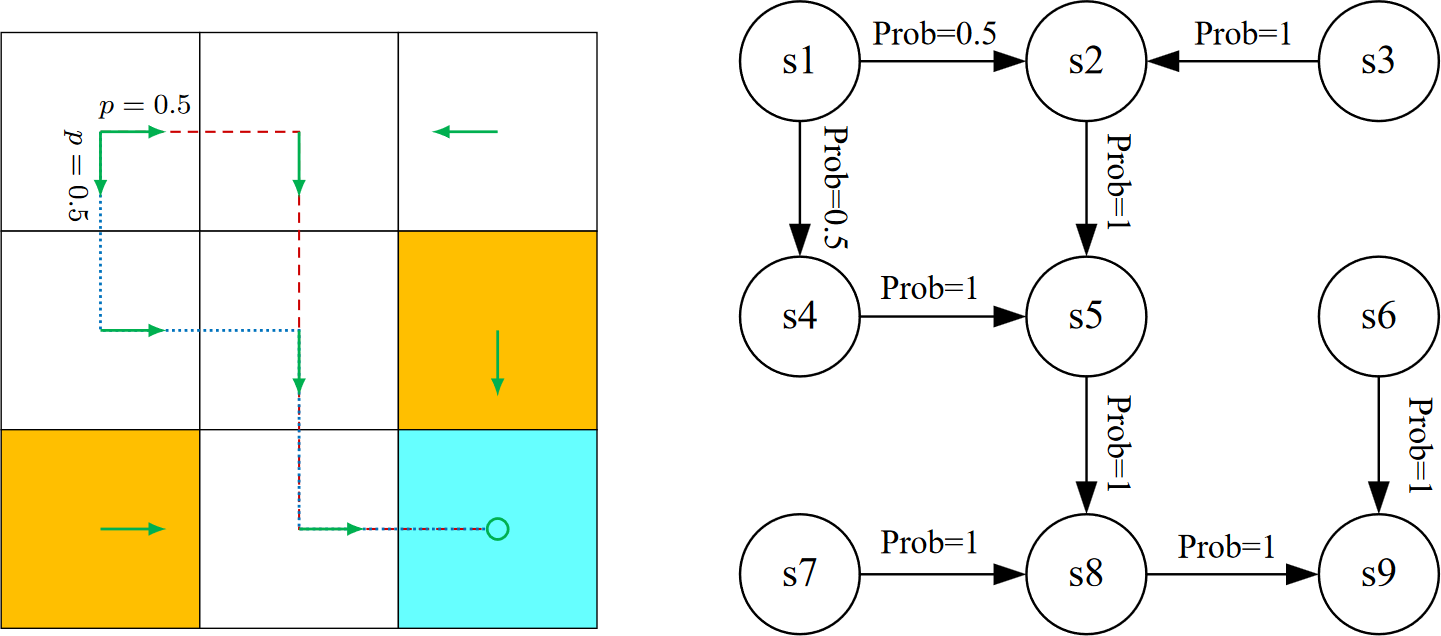
\includegraphics[width=.75\textwidth]{figures/ch3/3.mdp.png}
    \caption{The example grid as a Markov Process graph, where the nodes
    represent the states and the edges represent the state transitions.}
    \vspace{-10px}
    \caption*{\scriptsize{Source: \cite{zhao2024RLBook}}}
    \label{fig:mdp}
\end{figure}


\subsection{Reinforcement Learning Algorithms}

In \cite{openaiPartKinds}, the landscape of algorithms in modern reinforcement
learning is explored.

The algorithms used in reinforcement learning almost always rely on
\textbf{value functions}.
The \textbf{value} is the expected return if the agent starts in
that state or state-action pair and then follows a specific policy indefinitely.

\vspace{5cm}

There are four primary value functions to consider:

\begin{itemize}
    \item \textbf{On-Policy Value Function, \( V^{\pi}(s) \)}: This function
    represents the expected return if the agent starts in state \( s \)
    and acts according to the policy \( \pi \):
    $$ V^{\pi}(s) = \mathbb{E}_{\tau \sim \pi} \left[ R(\tau) \mid s_0 = s \right] $$
    \item \textbf{On-Policy Action-Value Function, \( Q^{\pi}(s,a) \)}:
    This function gives the expected return if the agent starts in state \( s \),
    takes an arbitrary action \( a \), and then always follows the policy \( \pi \):
    $$ Q^{\pi}(s,a) = \mathbb{E}_{\tau \sim \pi} \left[ R(\tau) \mid s_0 = s, a_0 = a \right] $$
    \item \textbf{Optimal Value Function, \( V^*(s) \):} This function provides
    the expected return if the agent starts in state \( s \) and follows the
    optimal policy for the environment:
    $$ V^*(s) = \max_{\pi} \mathbb{E}_{\tau \sim \pi} \left[ R(\tau) \mid s_0 = s \right] $$
    \item \textbf{Optimal Action-Value Function, \( Q^*(s,a) \):} This function
    represents the expected return if the agent starts in state \( s \),
    takes an arbitrary action \( a \), and then follows the optimal policy for the environment:
    $$ Q^*(s,a) = \max_{\pi} \mathbb{E}_{\tau \sim \pi} \left[ R(\tau) \mid s_0 = s, a_0 = a \right] $$
\end{itemize}

Figure \ref{fig:mdp}
presents a partial taxonomy of the modern reinforcement learning algorithms.
One key distinction is whether the agent utilizes (or learns) a model of
the environment. A model, in this context, refers to a function that predicts
state transitions and rewards.

\begin{figure}[h]
    \centering
    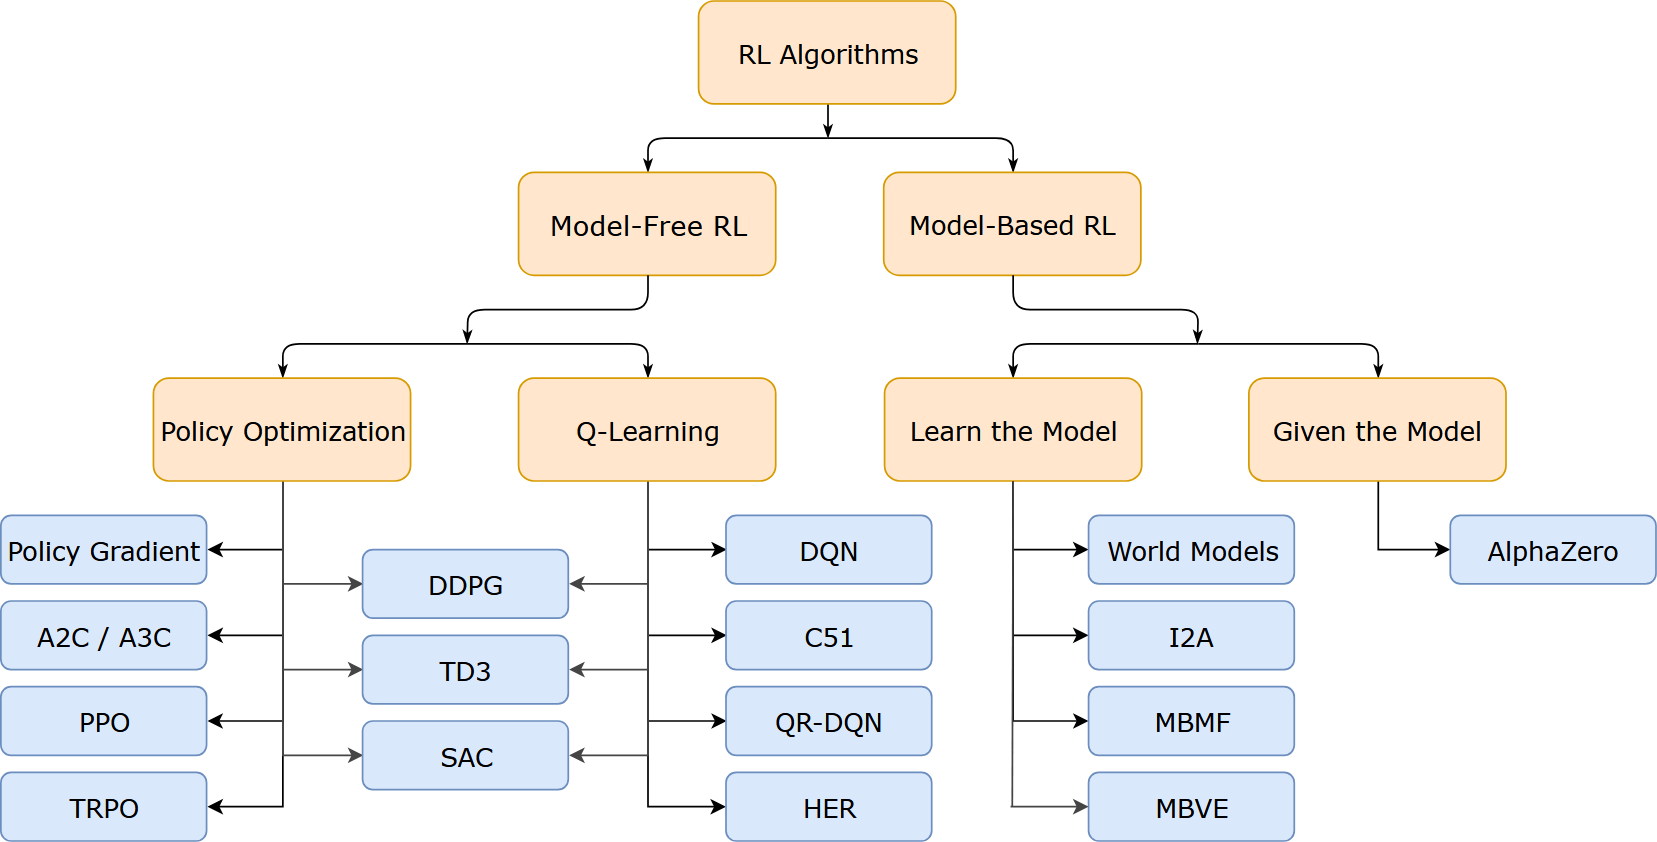
\includegraphics[width=.8\textwidth]{figures/ch3/4.rlalg.png}
    \caption{Partial taxonomy of algorithms in modern RL.}
    \vspace{-10px}
    \caption*{\scriptsize{Source: \cite{openaiPartKinds}}}
    \label{fig:mdp}
\end{figure}

The primary advantage of having a model is that it enables the agent
to plan by predicting future states and rewards.
However, the major drawback is that an accurate model of the environment
is often unavailable to the agent.
Algorithms which use a model are known as \textbf{model-based} methods,
while those that do not are referred to as \textbf{model-free} methods.
Our focus will be on the latter.

Model-free methods can be categorized into two main approaches
for representing and training agents:
\begin{itemize}
    \item \textbf{Policy Optimization:} explicitly represents a policy
    as \( \pi_{\theta}(a \mid s) \) and optimizes the parameters \( \theta \)
    either directly via gradient ascent on the performance objective
    \( J(\pi_{\theta}) \) or indirectly by maximizing local approximations
    of \( J(\pi_{\theta}) \).
    Typically, this optimization is performed \textbf{on-policy},
    meaning that each update uses data collected while the agent is acting
    according to the most recent version of the policy.

    \item \textbf{Q-Learning:} involves learning an approximator
    \( Q_{\theta}(s,a) \) for the optimal action-value function \( Q^*(s,a) \).
    Unlike policy optimization, Q-learning is generally performed \textbf{off-policy},
    allowing updates to use data collected at any time during training,
    irrespective of the agent's policy at the time of data collection.
    The corresponding policy is derived from the relationship between
    \( Q^* \) and \( \pi^* \), where the actions taken by the Q-learning
    agent are determined by
    $$ a(s) = \arg \max_a Q_{\theta}(s,a) $$
    An example of a Q-learning algorithm is Deep Q-Network (\textbf{DQN}),
    which uses a deep neural network to approximate the optimal action-value
    function in environments with large state spaces,
    and its variants such as Double DQN (\textbf{DDQN}) and
    Dueling Double DQN (\textbf{D3QN}).

\end{itemize}

There are also hybrid approaches that combine elements
of both policy optimization and Q-learning.
In this spectrum of algorithms we can find 
\textbf{actor-critic methods}, which consist of two components:
an \textbf{actor} that makes actions and a \textbf{critic} that evaluates them.
An example of an actor-critic algorithm is Twin-Delayed DDPG (\textbf{TD3}).

If samples are collected during training the reinforcement learning is
considered \textbf{online}, otherwise,
if the training set is fixed, it is \textbf{offline}.

\section{Causal Inference}

\cite{Neal_2020a}

\section{Generative Adversarial Networks}

\chapter{Methodology}

\chapter{Experiments}

\chapter{Conclusion}

\appendix

%\chapter{Questa è un'appendice}

\lipsum[5]

\section*{Questa è un'altra sezione, ma non viene inserita nell'indice}

\lipsum[6] Grazie, Lo Spazio.


\bibliographystyle{apalike}
\bibliography{chapters/Bibliografia.bib}

\end{document}
% -----------------------------------------------------------------
